\chapter{Datenanalyse}
Für die Auswertung eines Fragebogens gibt es verschiedene Methoden die zum Einsatz kommen können. Der hier verwendetet Fragebogen verwendet drei arten von Antwortmöglichkeiten
\begin{itemize}
	\item[Typ 1:] {Ordinalskala: Antworten mit einer Rangfolge\\
		(z.B. sehr nützlich, etwas nützlich oder unnütz)\\
		Fragen 1, 3, 4, 6, 8 und 9}
	\item[Typ 2:] {Nominalskala: Antworten ohne Rangfolge\\
		(z.B. PC, Tablett und Mobile)\\
		Fragen 2 und 10}
	\item[Typ 3:] {Freie Antworten \\
		Fragen 5, 7 und 10 (Sonstiges)}
\end{itemize}
Für die Verschiedenen Typen gibt es jeweils eine Verfahren zur Bewertung.
Typ 1 und 2 werden mit der Häufigkeitsmethode ausgewertet, wobei bei Typ 1 auch noch nach Rangfolge ausgewertet werden kann. Bei Typ 3 kommt eine Qualitative Methode zum Einsatz.

Da für die Auswertung maximal nur 10 Datenpunkte zu Verfügung stehen, können keinen statistischen verfahren verwendet werden.

\subsection{Aufbereitung von surveymonkey.de}
Die Webseite www.surveymonkey.de bereitet die Ergebnisse passend auf. Die vom Typen 1 und 2 sind jeweils Tabellarisch als auch mit einem Balkendiagramm dargestellt.
Die von Antworten zu Typ 3 sind in einer Tabelle zur weiteren Auswertung Festgehalten.

Da ein Export nur für zahlenden Kunden angeboten wird, müssen die Daten manuelle kopiert und per Screenshot gesichert werden.

Ein erste Überblick zeigt bereits, dass die Bewertungen überwiegend positiv ausgefallen sind.

\subsection{Die Daten}
\begin{wrapfigure}{r}{0.4\textwidth}
	\centering
	\fbox{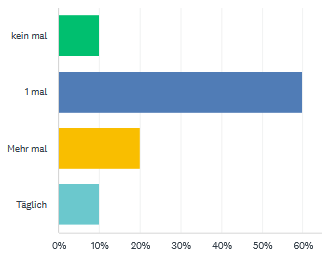
\includegraphics[width=0.30\textwidth]{images/frage-01}}
\end{wrapfigure}
Bei Frage 1 haben 6 von 10 angeben das sie die DHBW Star nur einmal in den letzten 7 Tagen genutzt haben. Es ist zu vermuten dass sich die meiste die Seite einmal Angeschaut haben, aber sich bereits so sehr an die bisherigen Informationsquellen gewohnt haben, dass sie keinen Grund sagen sich für die letzten Wochen um zu gewöhnen.

Auf die Frage Wie nützlich die Startseite empfunden wird, hat nur 1 Person unnütz angegeben. 
Auch bei den Frage zum \emph{Scheduler} und \emph{Food} gaben 8 von 10 Personen an dass ihnen die DHBW-Star besser oder viel besser gefällt.
2 Personen 
\begin{wrapfigure}{r}{0.4\textwidth}
	\centering
	\fbox{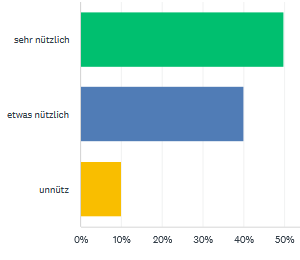
\includegraphics[width=0.30\textwidth]{images/frage-02}}
\end{wrapfigure}




 \cite{fragebogenKallus}, \cite{fragebogenRolf}, \cite{bachelorprint}